\chapter{Project 6: Web}

\section{Overview}
There's one piece of hardware that we haven't talked about yet. The ESP32-C3 microcontroller has a
WiFi processor built in. We can make use of this to connect to the internet and pull in all kinds of
data or transmit data to other services! If you've ever heard the phrase "Internet of Things", this
is what they mean. Over the course of this project, you will:
\begin{itemize}
    \item Use the embedded WiFi processor to connect to the internet
    \item Make requests to free 3rd party API services to fetch live data
    \item Use the connected buttons and screen to display different sets of that data
\end{itemize}
At the end of this project, your microcontroller should run a MicroPython program that displays 3
different screens of data that you can rotate through with the buttons. Let's get started!
\begin{figure}[H]
\centering
    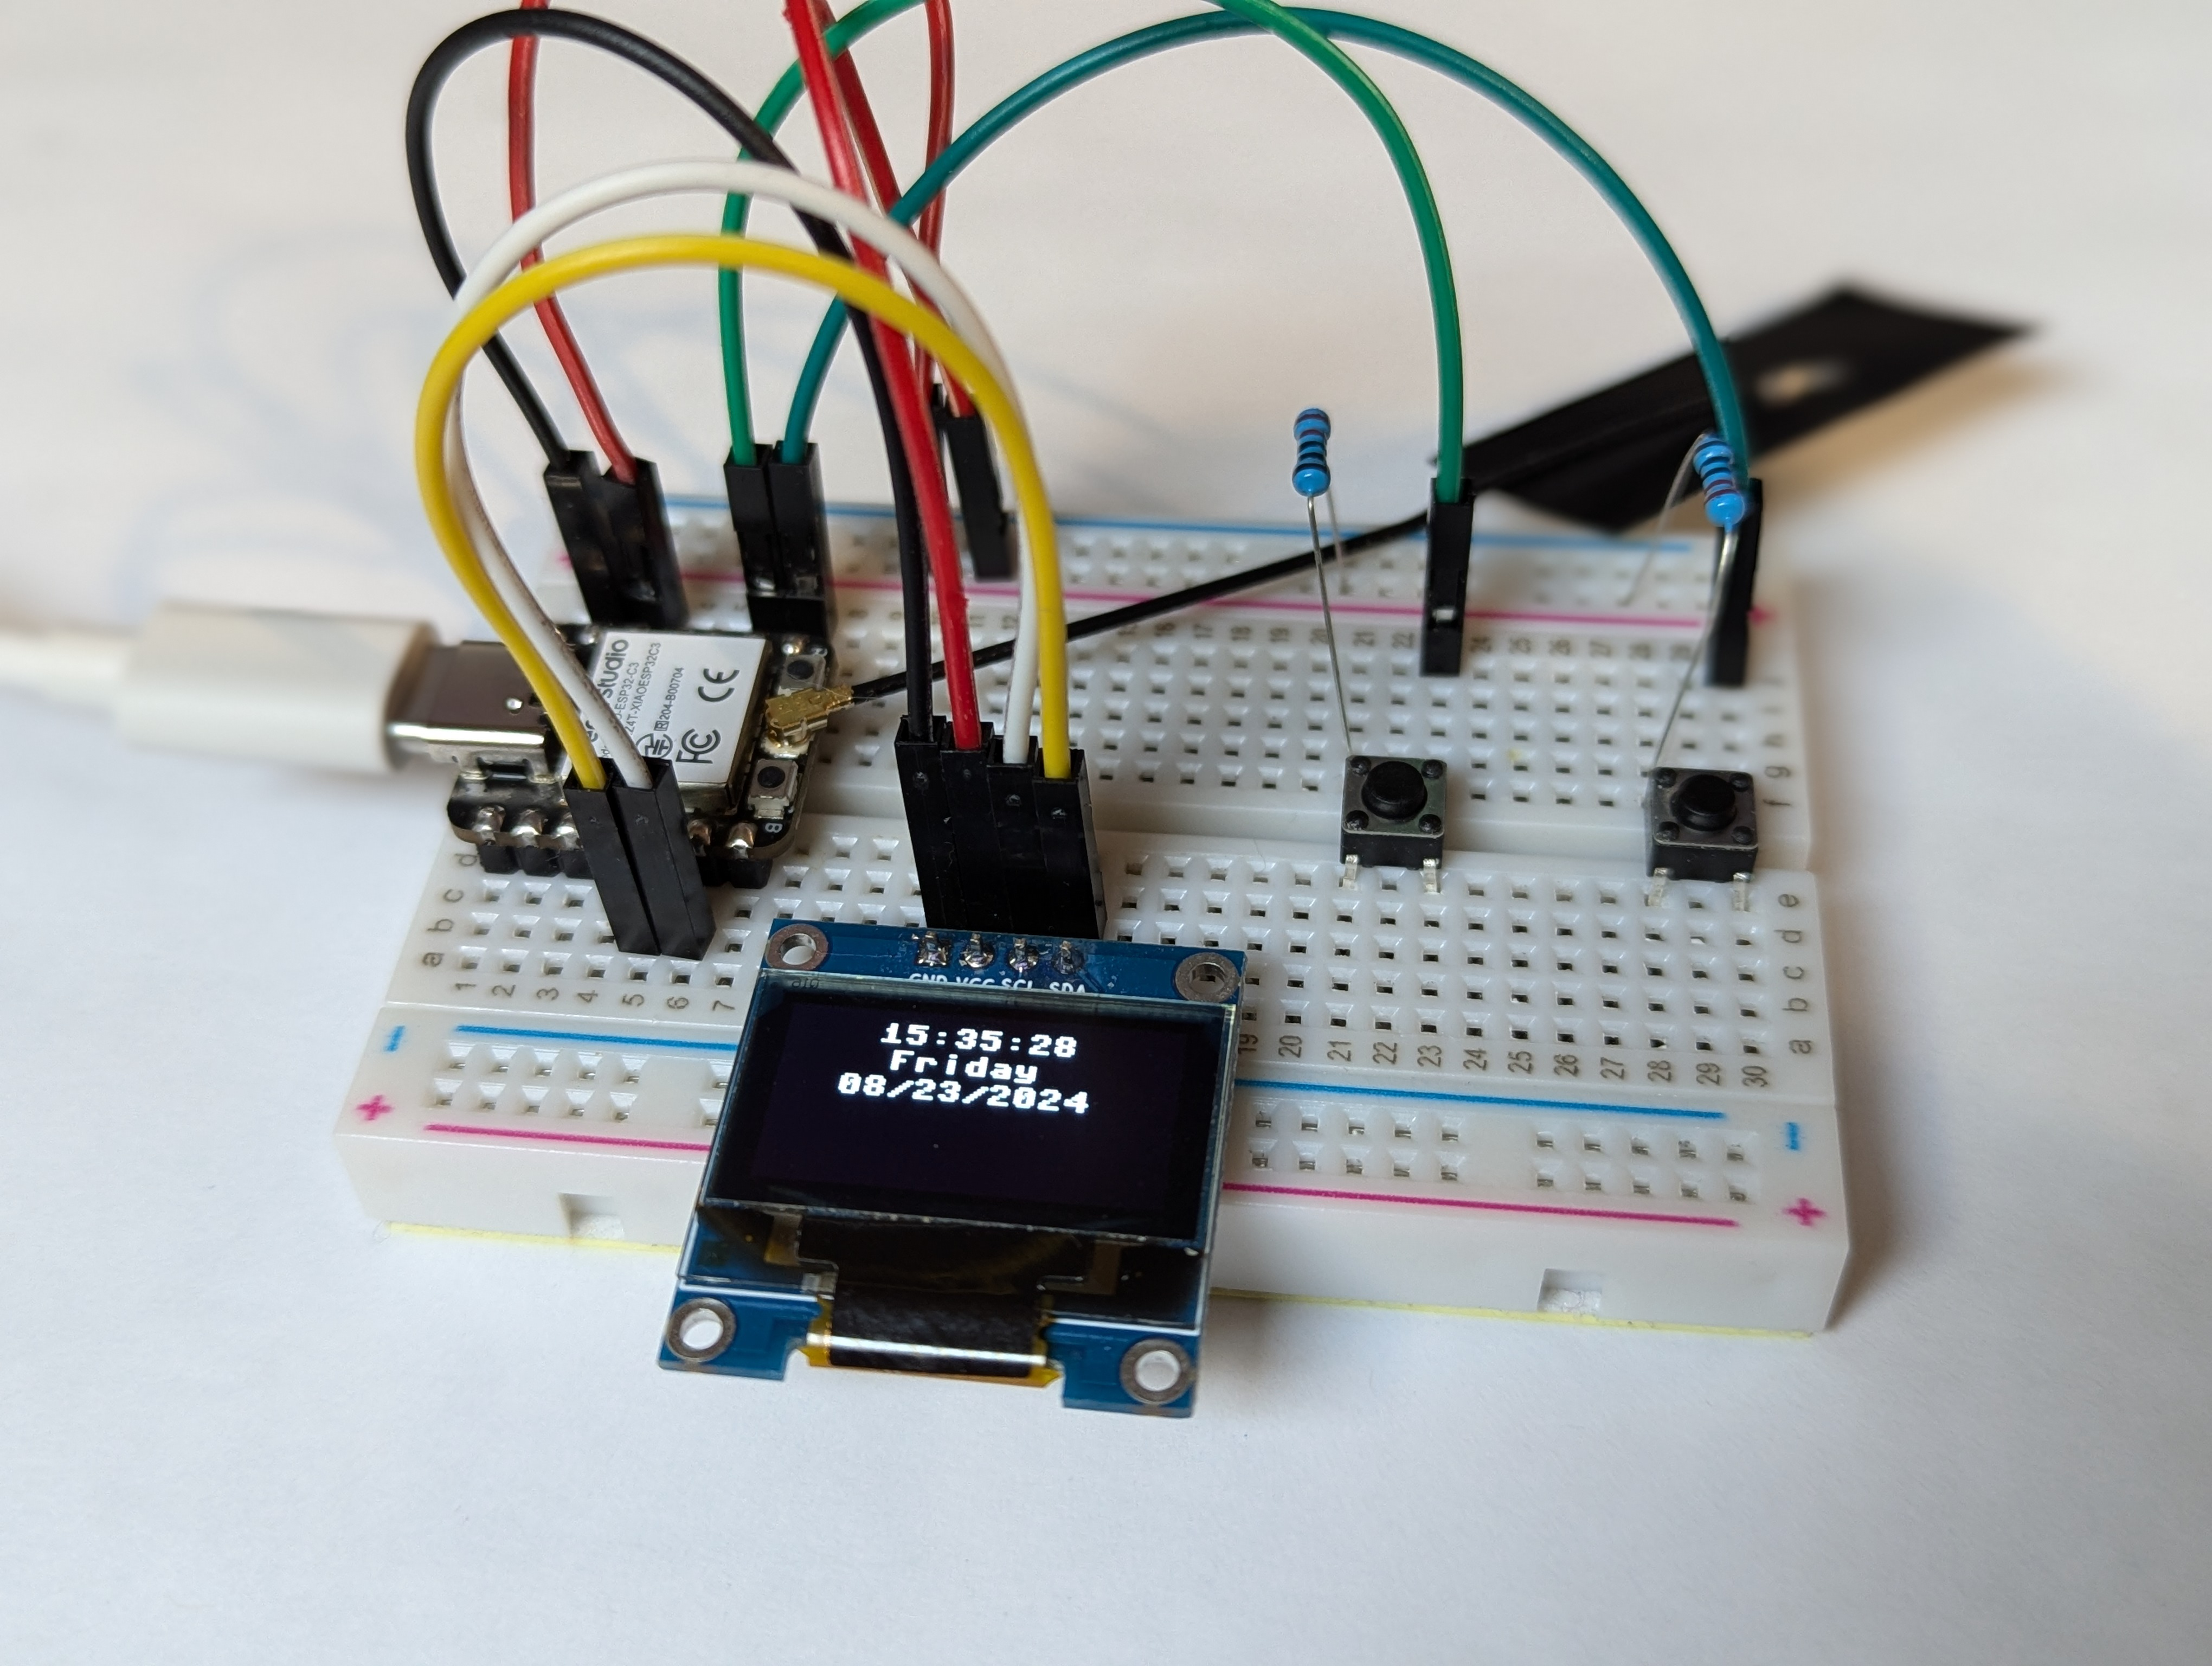
\includegraphics[width=.6\linewidth]{project_6/screen_connected.jpg}
    \caption{The end result should look something like this}
\end{figure}

\pagebreak

\section{Directions}

\subsection{Creating the circuit}
Using jumper cables, you will be assembling a circuit between your microcontroller, your breadboard, two
buttons and the small OLED screen included in your kit.

\subsubsection{Remove previous components}
Before beginning, remove any components from prior chapters including LEDs, buttons, and wires. You may leave the
microcontroller attached to the breadboard.

\subsubsection{Attach the microcontroller to the breadboard}
If it's not already, carefully insert the pins at the bottom of your microcontroller into the breadboard. Refer back
to \ref{pinout} for pin labels. When placing the board into the breadboard, make sure that the microcontroller is oriented such that:
\begin{itemize}
    \item The pin labeled \textbf{5V} is inserted in hole at \textbf{Column H, Row 1} of the breadboard (or \textbf{H1}, for short)
    \item The pin labeled \textbf{GPIO2} is inserted in hole \textbf{D1} of the breadboard
    \item The pin labeled \textbf{GPIO20} is inserted in hole \textbf{H7} of the breadboard
    \item the pin labeled \textbf{GPIO21} is inserted in hole \textbf{D7} of the breadboard
\end{itemize}
You may need to apply more pressure than expected to seat the microcontroller properly in the breadboard. When its over, it should look like this:
\begin{figure}[H]
    \centering
    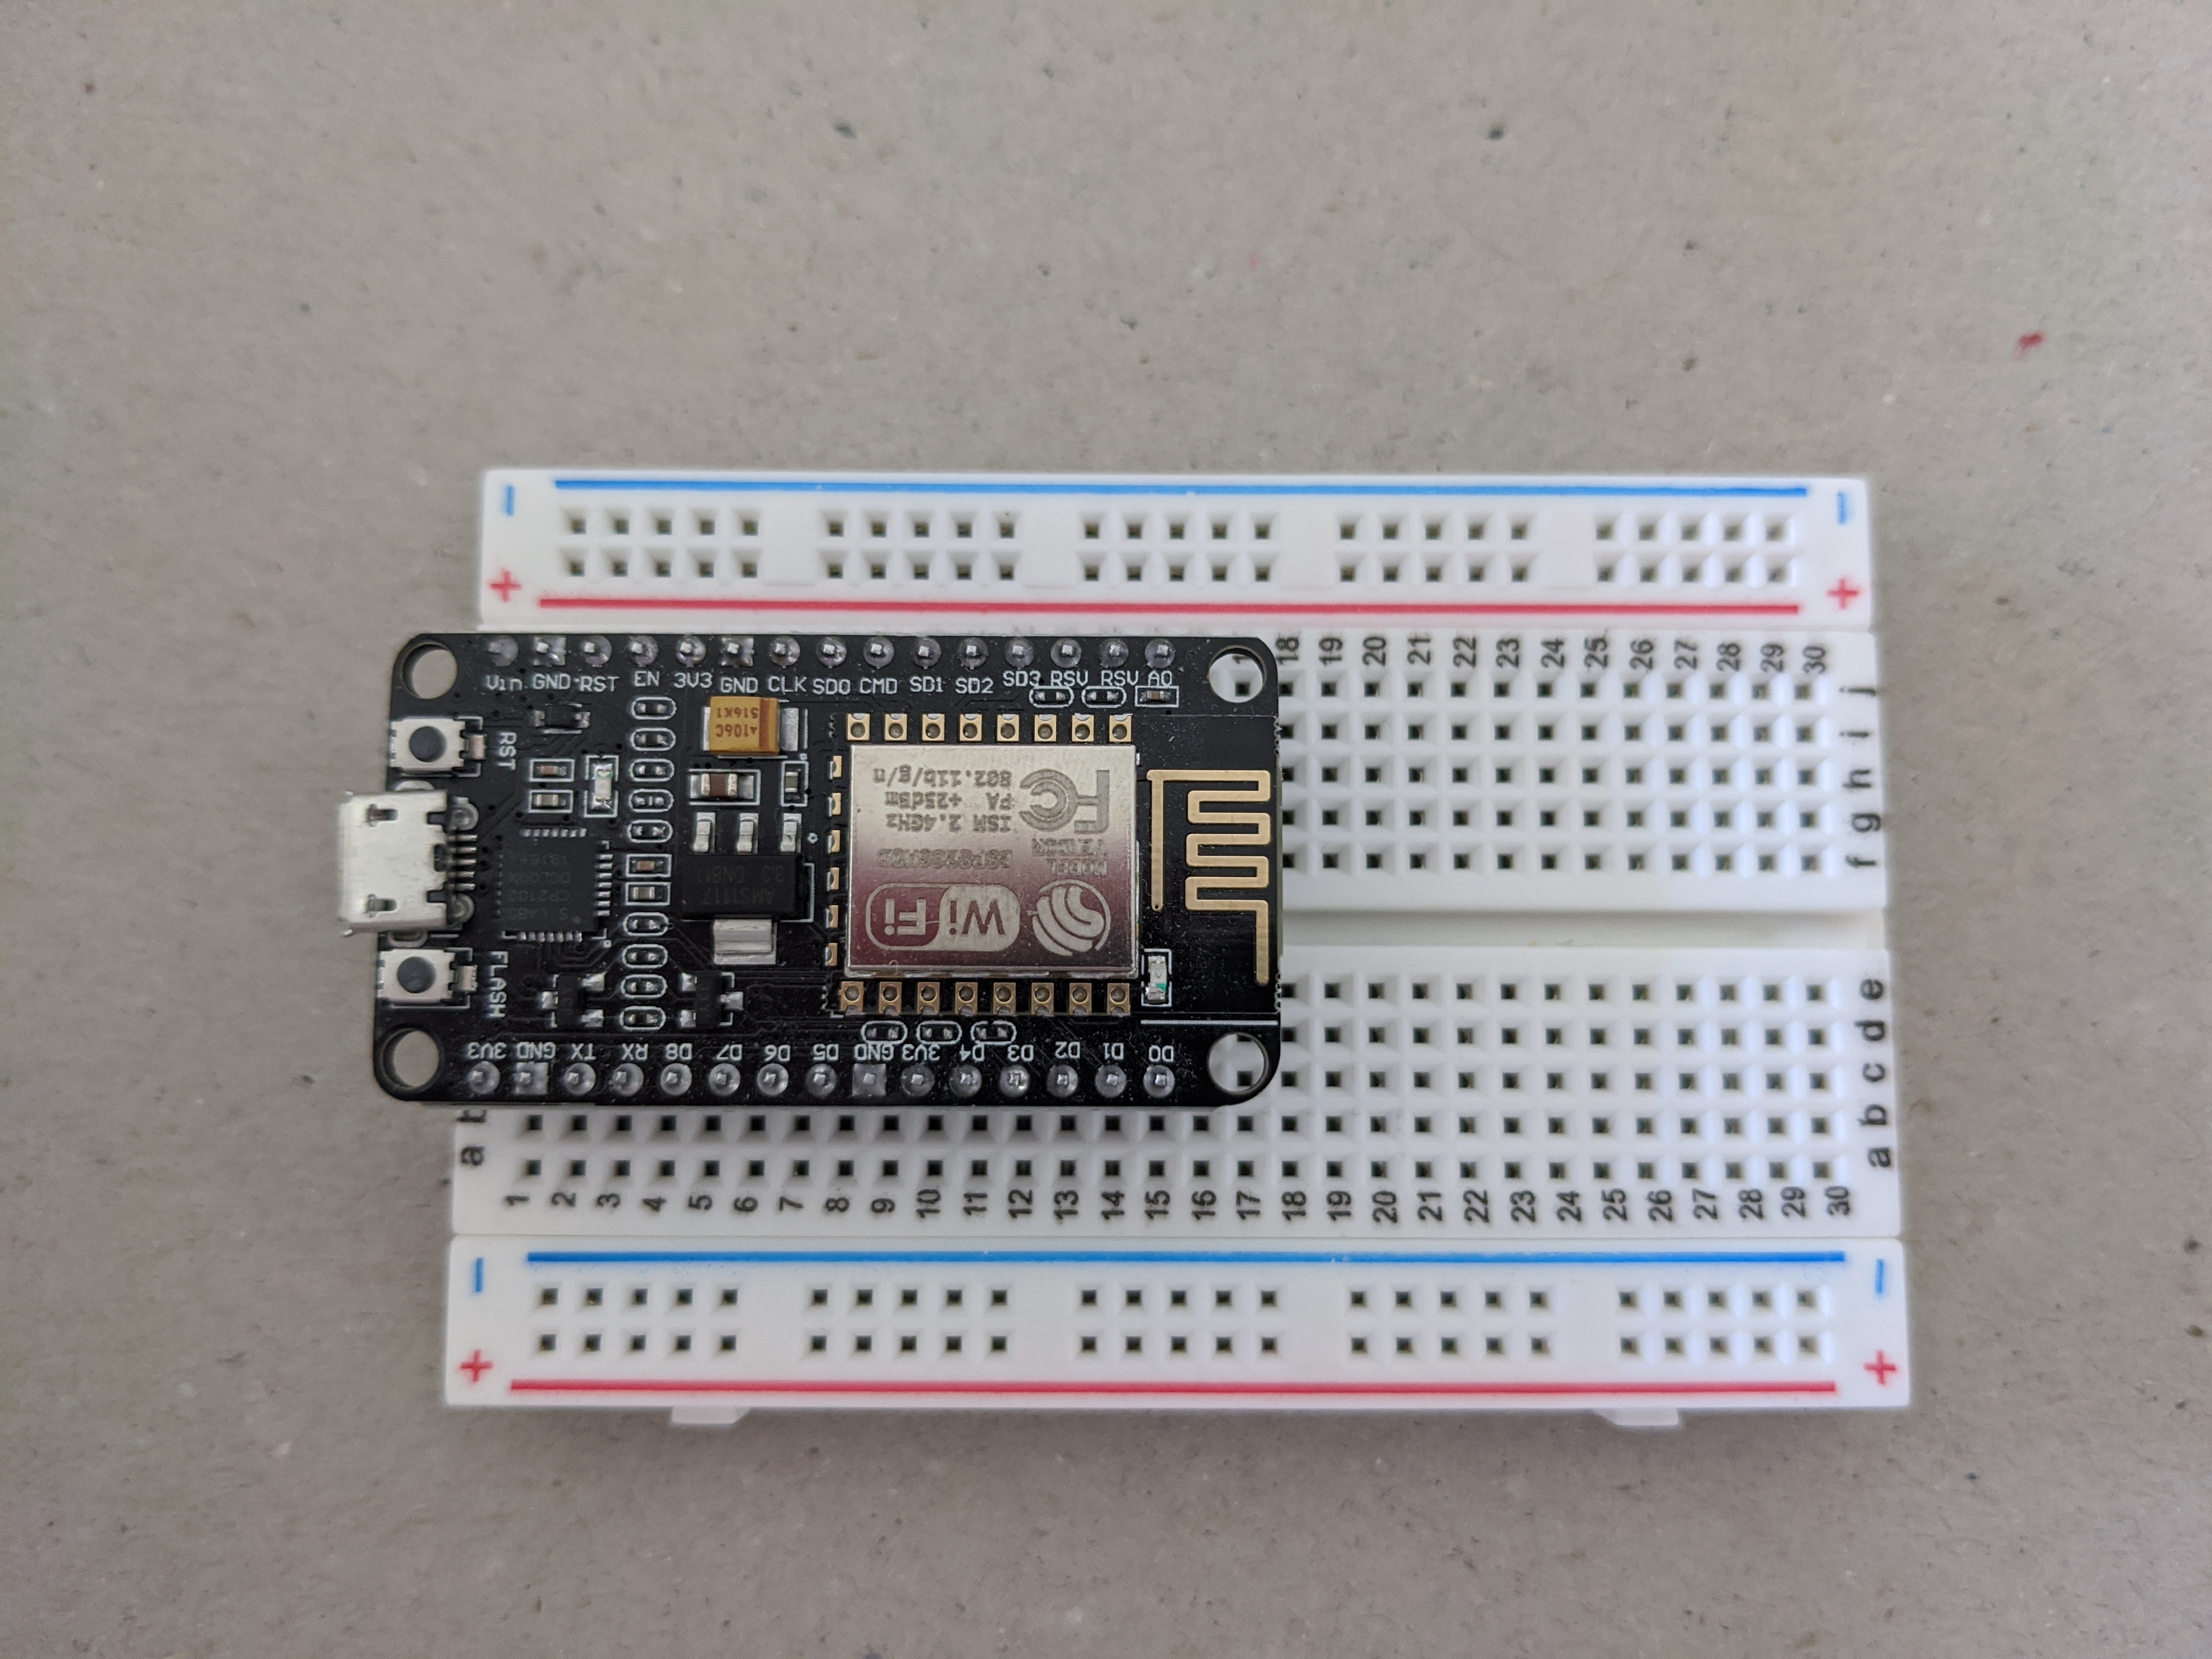
\includegraphics[width=.6\linewidth]{common/microcontroller_seated_in_breadboard.jpg}
    \caption{So far, so good!}
\end{figure}

\subsubsection{Place the OLED Screen and Buttons on the Board}
Place the buttons towards the right side of the breadboard. Then connect a resistor for each button between the top positive
bus (the red one) and the top left side of each button. Finally, place the OLED screen into the breadboard. Connect
it's 4 pins into holes \textbf{A12}, \textbf{A13}, \textbf{A14}, and \textbf{A15}.

You should be left with something that looks like this:
\begin{figure}[H]
    \centering
    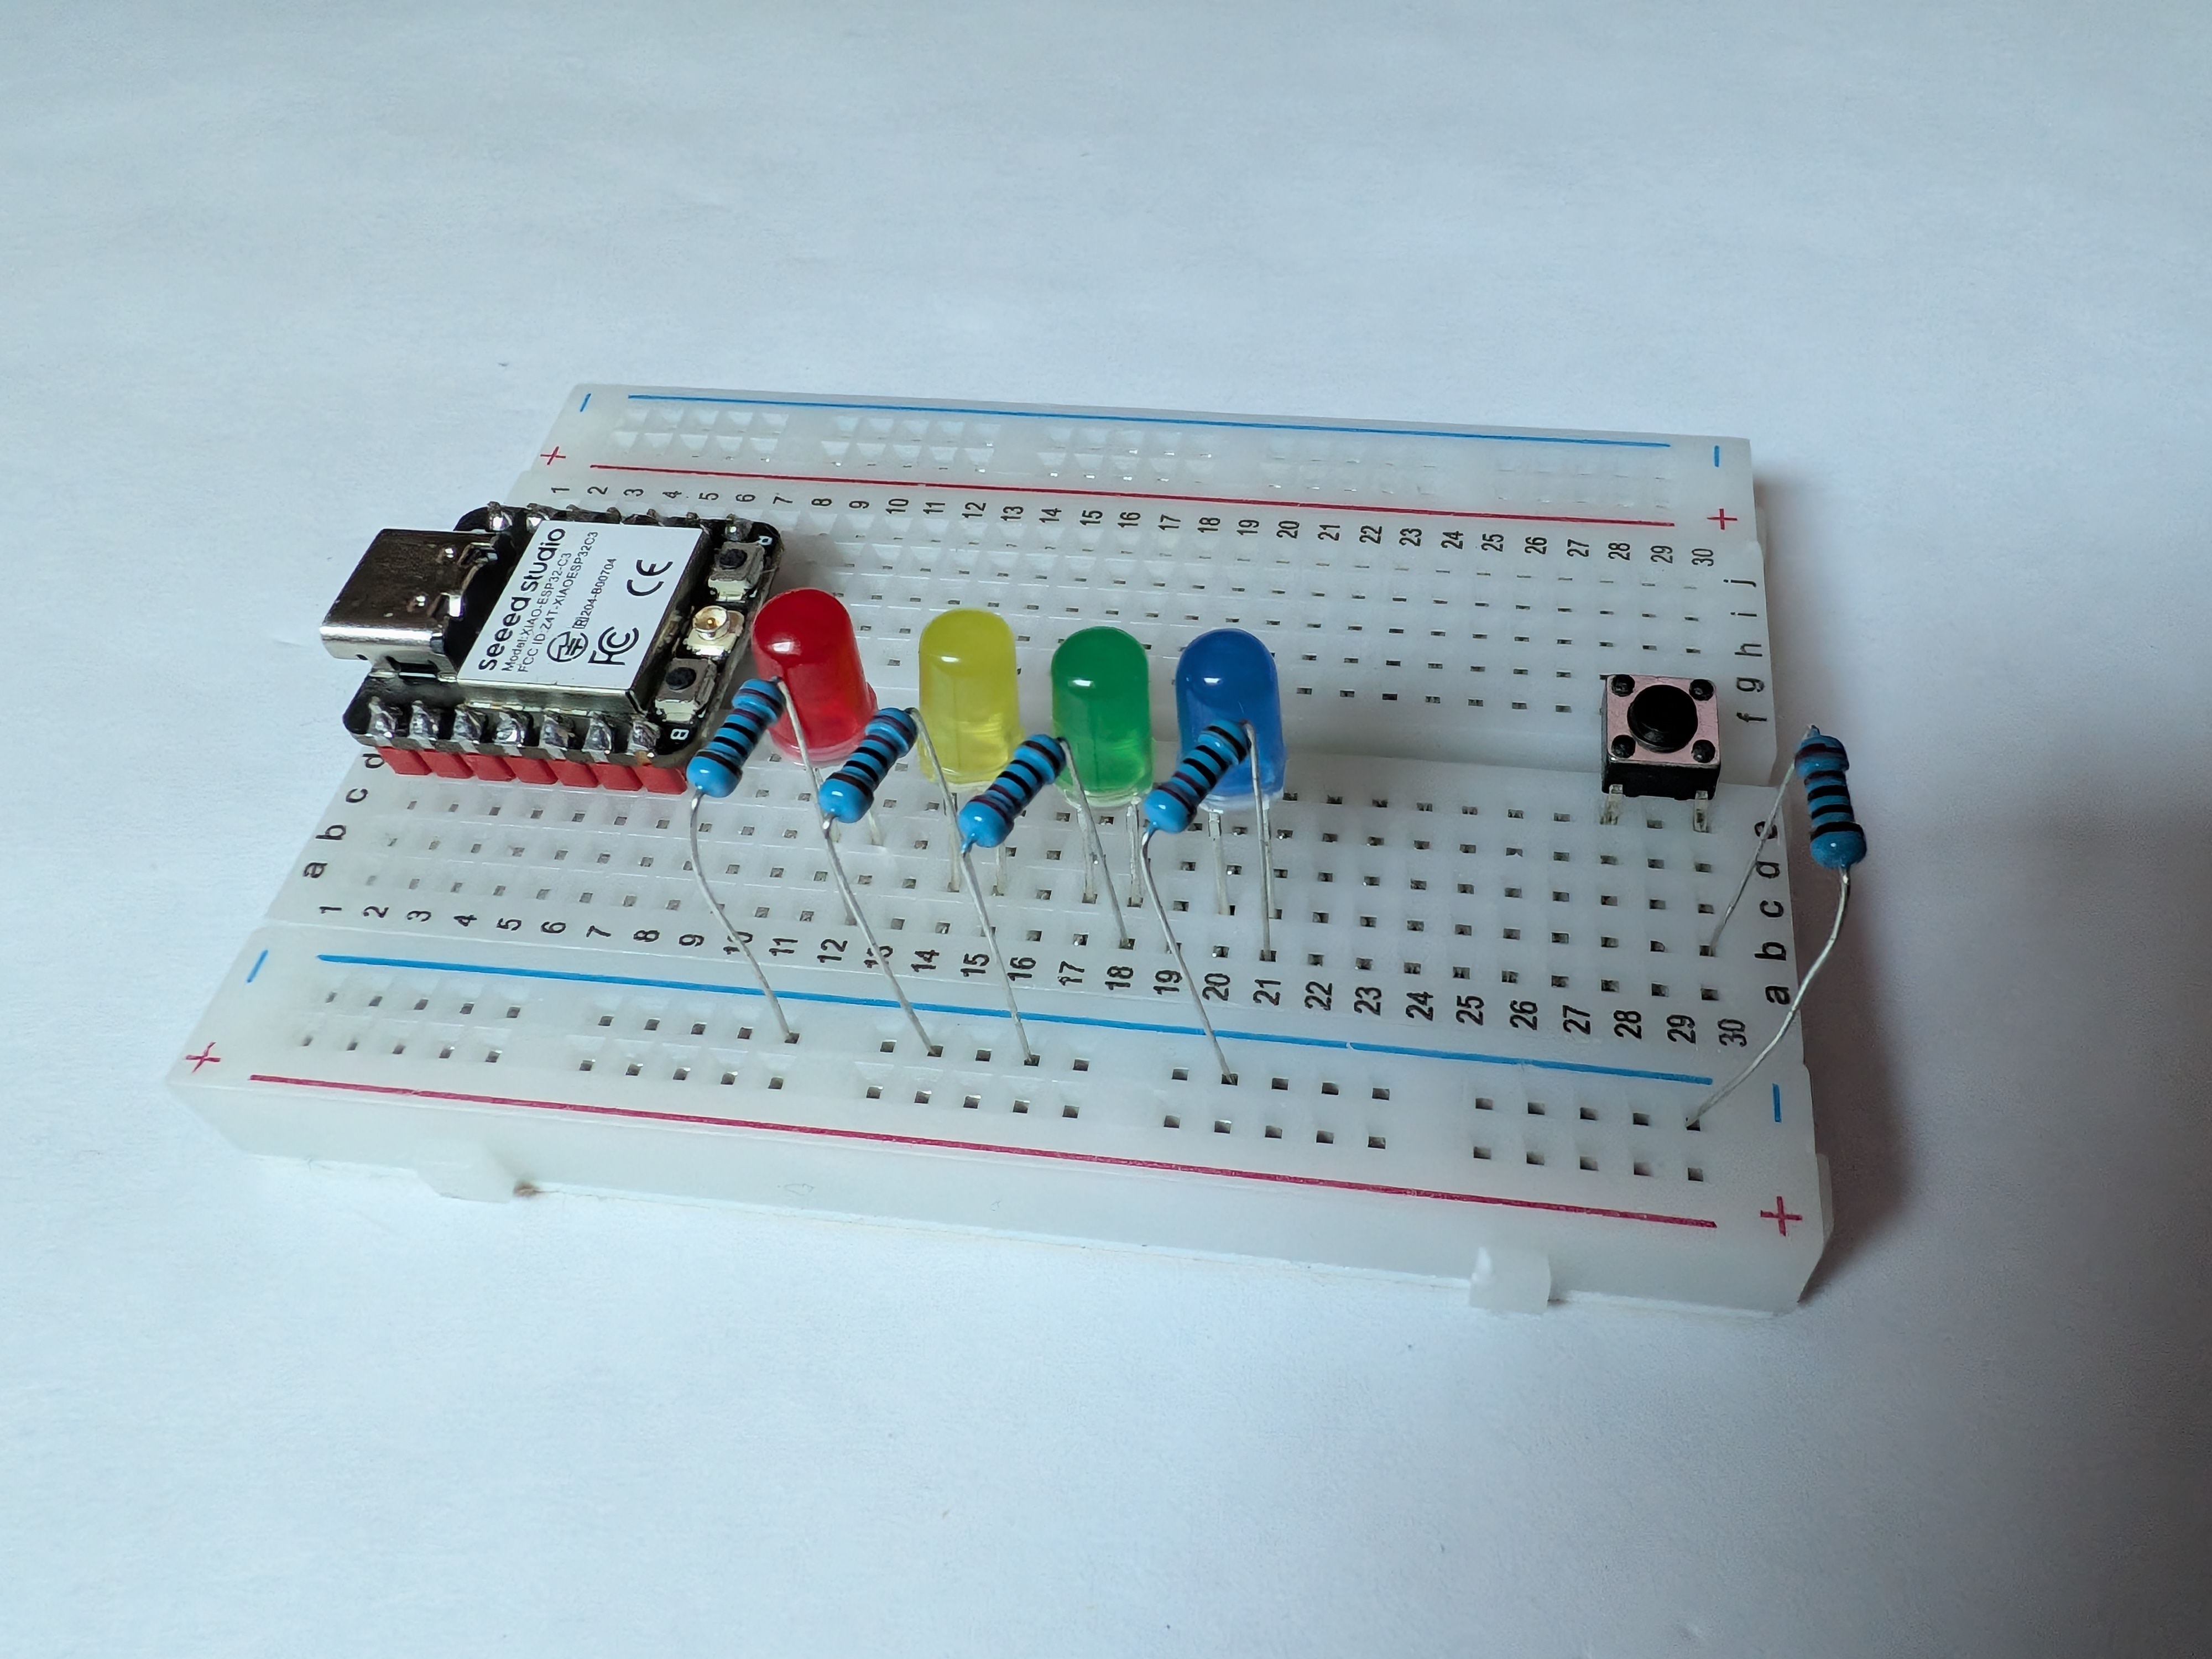
\includegraphics[width=.6\linewidth]{project_6/components_placed.jpg}
    \caption{All of the components except for the jumper wires are now placed.}
\end{figure}

\subsubsection{Connect the necessary jumper wires}
\begin{itemize}
    \item Place one end of a red jumper wire into hole \textbf{I22} of the breadboard and the other end into
    any hole on the top positive bus (the red one). This will provide \textbf{3.3} volts of power to all of the components.
    \item Using a black jumper wire, place one end of the wire into hole \textbf{I21} of the breadboard and the other
    end into \textbf{C12}, which is the pin marked as GND on the OLED.
    \item Place a red jumper wire between the top positive bus and hole \textbf{C13}. This will provide power for the OLED screen.
    \item Place a white jumper wire between \textbf{C14} and \textbf{B25}. This will provide a clock signal to the OLED screen.
    \item Place a yellow jumper wire between \textbf{C15} and \textbf{B24}. This will provide the data to display on the OLED screen.
    \item Place a green jumper wire between \textbf{J23} and \textbf{J6}. This will provide the signal to move to the previous screen.
    \item Place a green jumper wire between \textbf{J30} and \textbf{J7}. This will provide the signal to move to the next screen.
    \item Finally, attach the antenna to the microcontroller by plugging the gold end of its wire into the socket in the bottom of
    the microcontroller's board, between the buttons.
\end{itemize}

You should be left with something that looks like this:
\begin{figure}[H]
    \centering
    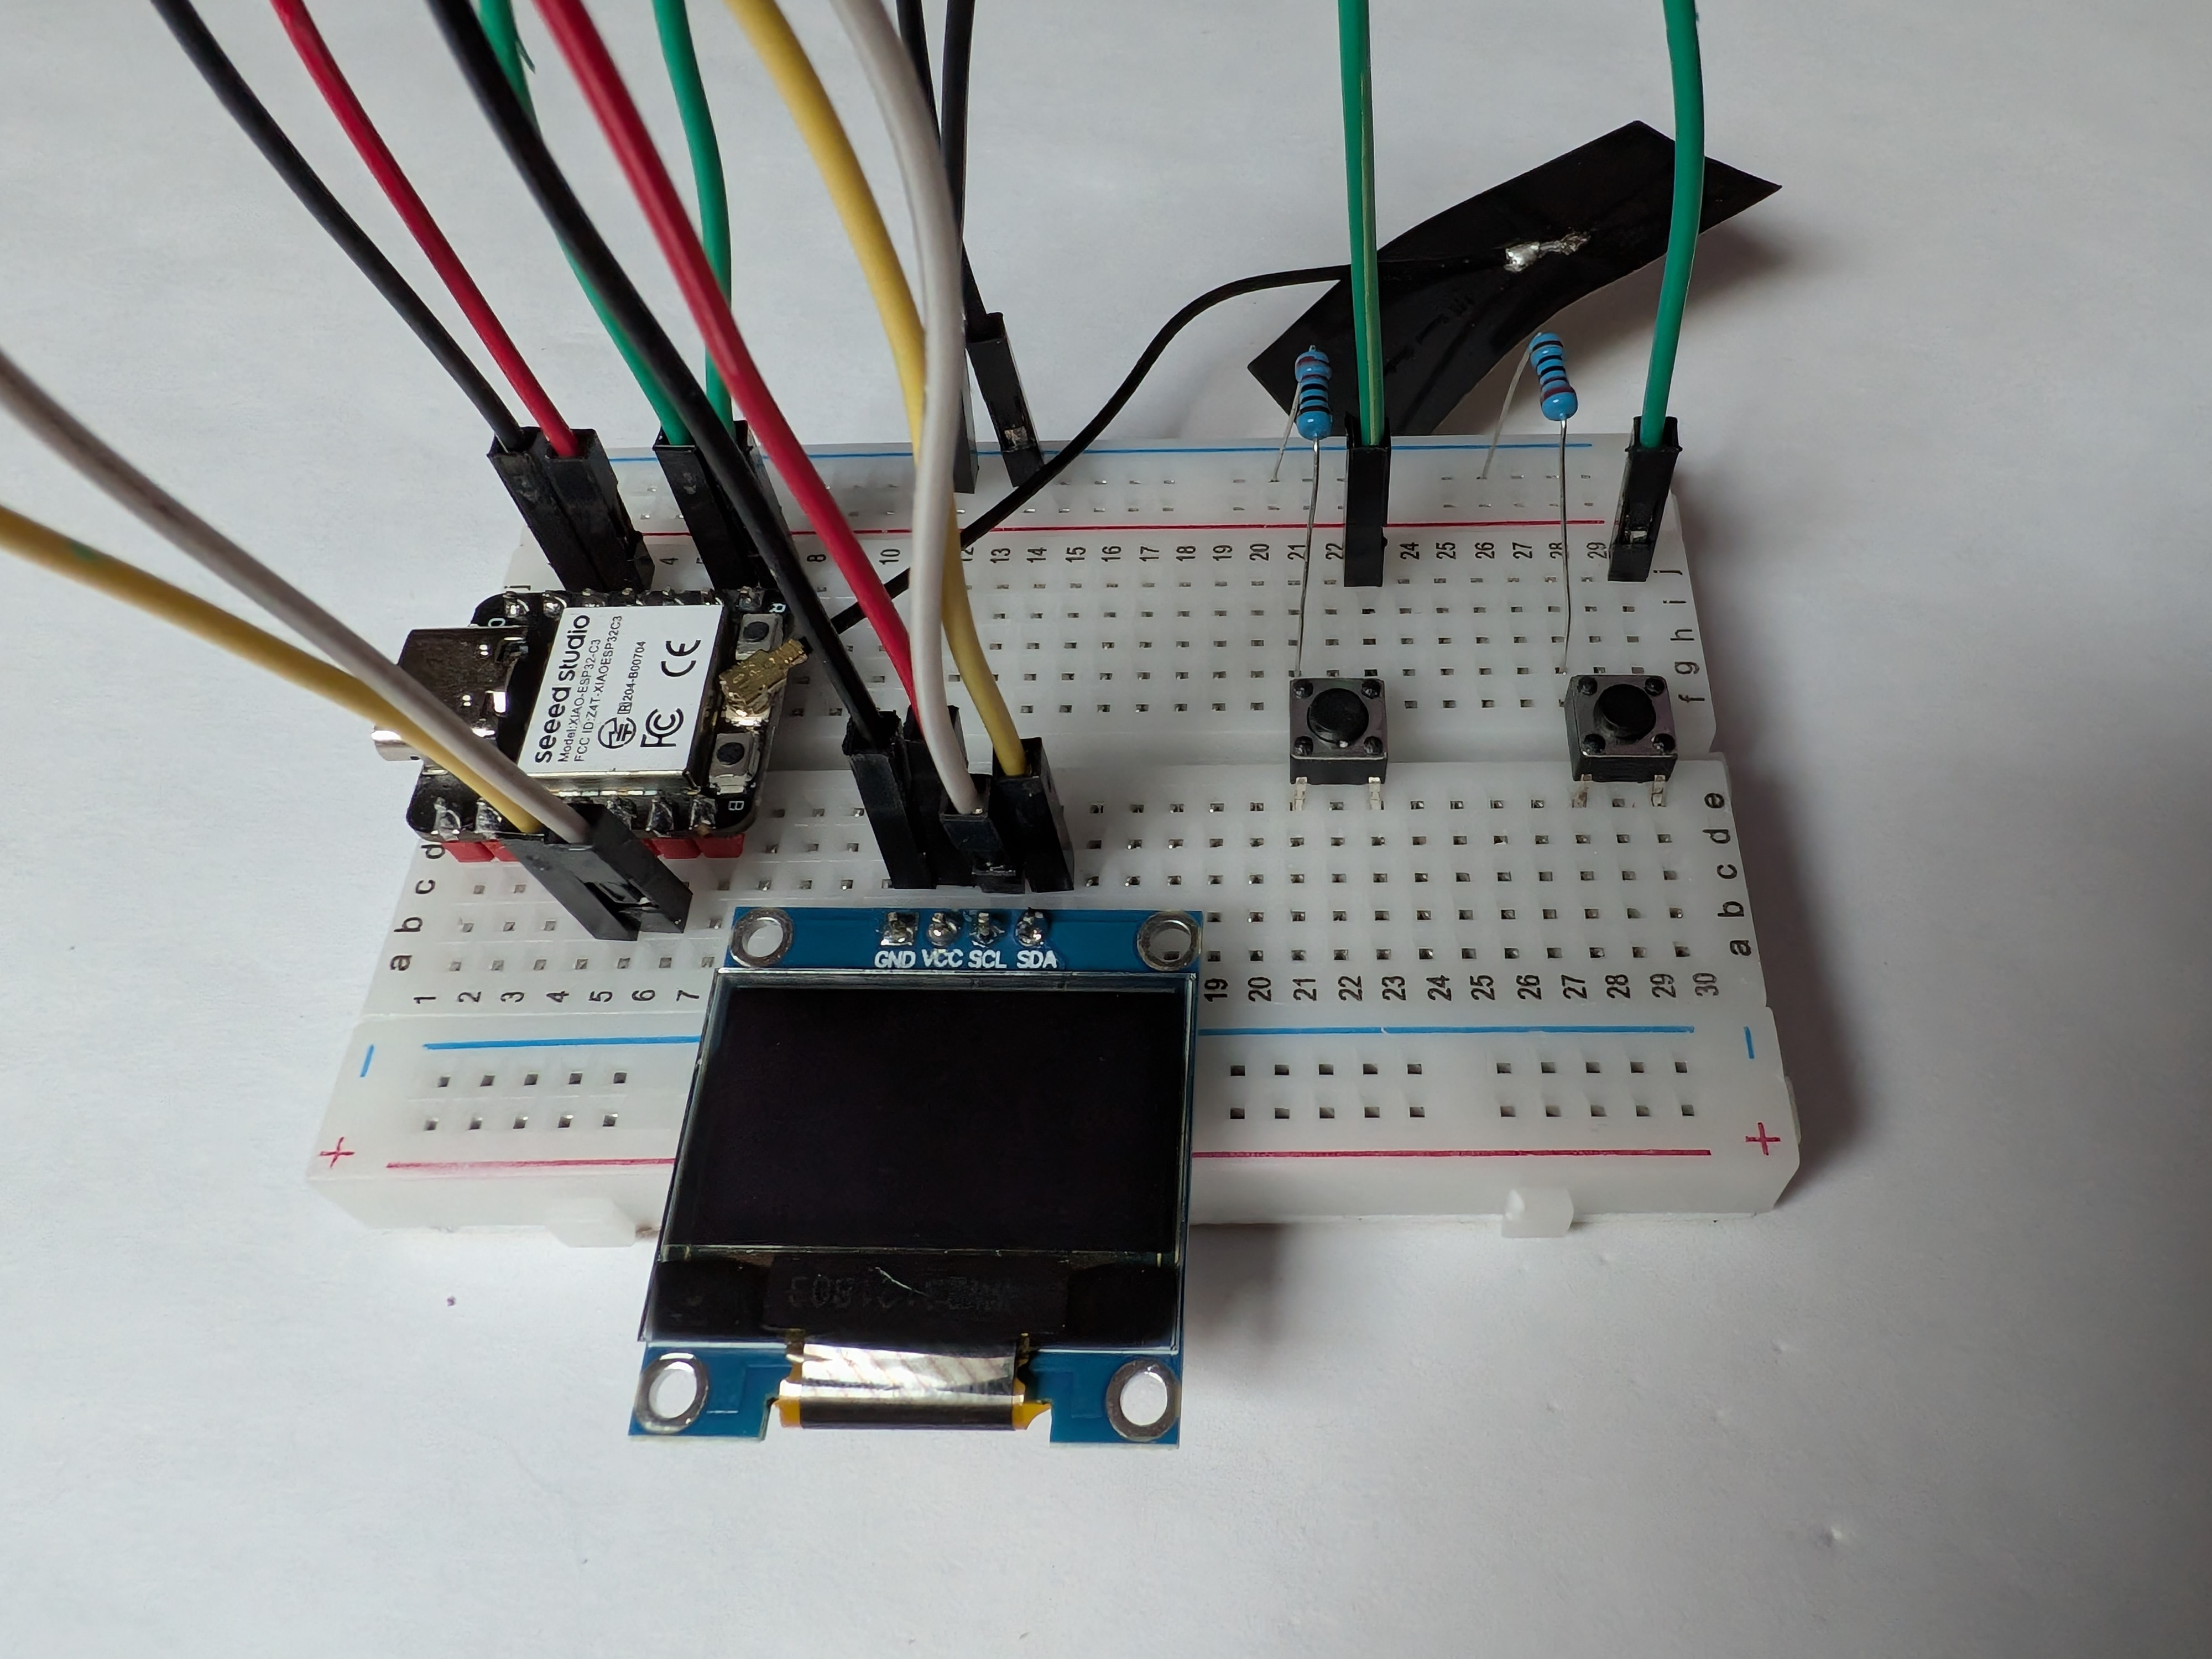
\includegraphics[width=.6\linewidth]{project_6/wired_up.jpg}
    \caption{All components and wires are now installed}
\end{figure}

\subsection{Programming the microcontroller}
Once all of the wiring is correct, connect the USB cable to the microcontroller (you will want to push the cable underneath the
two resistors on the left) and go to https://viper-ide.org/ in your computer's web browser. Click on the USB icon in the top
right and choose your microcontroller from the list:

\begin{figure}[H]
    \centering
    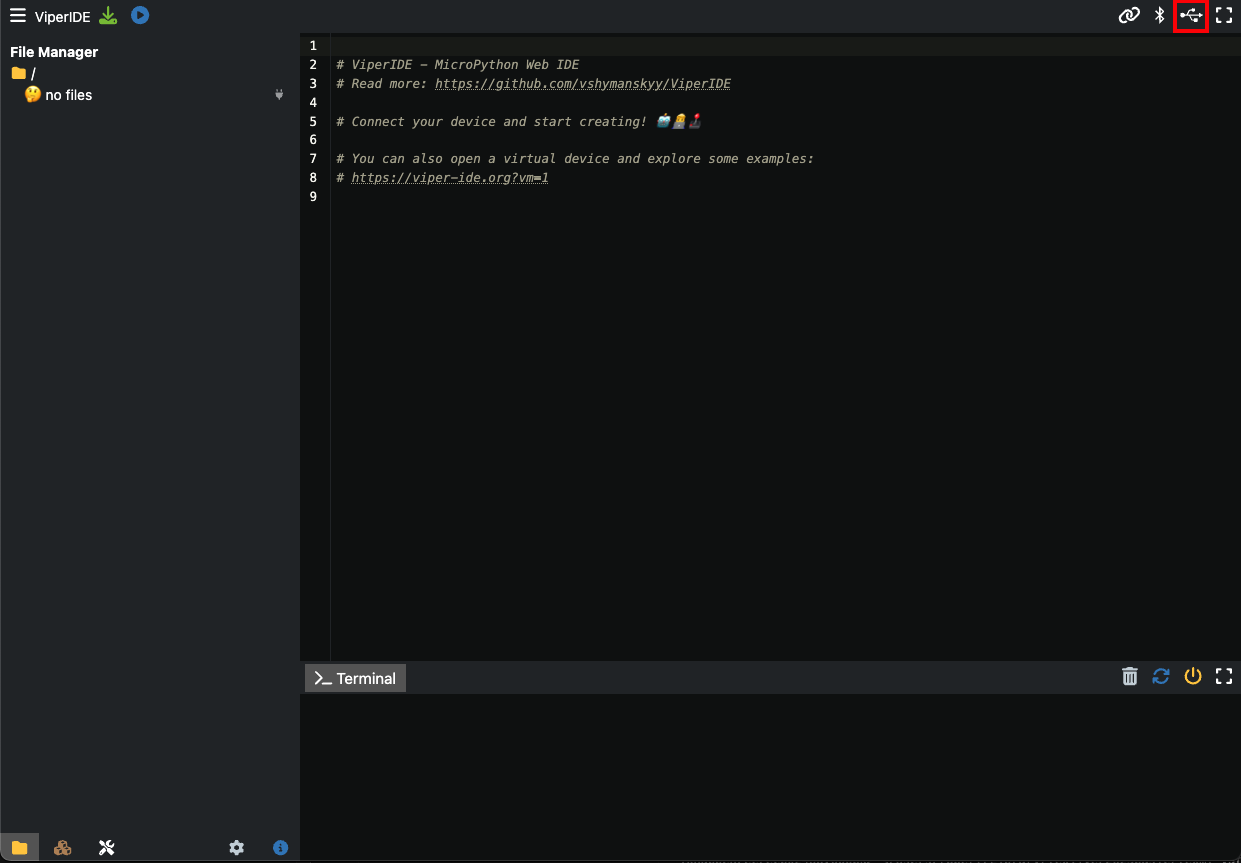
\includegraphics[width=.6\linewidth]{common/viper_ide_usb_connect.png}
    \caption{Click the button highlighted in red.}
\end{figure}

If you see multiple items in the dialog that pops up, choose the one that starts with "USB JTAG". See below for an example:
\begin{figure}[H]
    \centering
    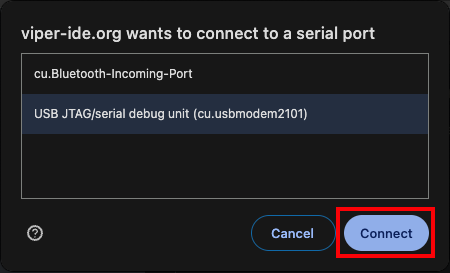
\includegraphics[width=.6\linewidth]{common/viper_ide_usb_choice_connect.png}
    \caption{Click the button highlighted in red.}
\end{figure}

Once you have connected, you will see a green dialog labeled "Device connected" and the file manager on the list
will populate with the list of files installed on the device:
\begin{figure}[H]
    \centering
    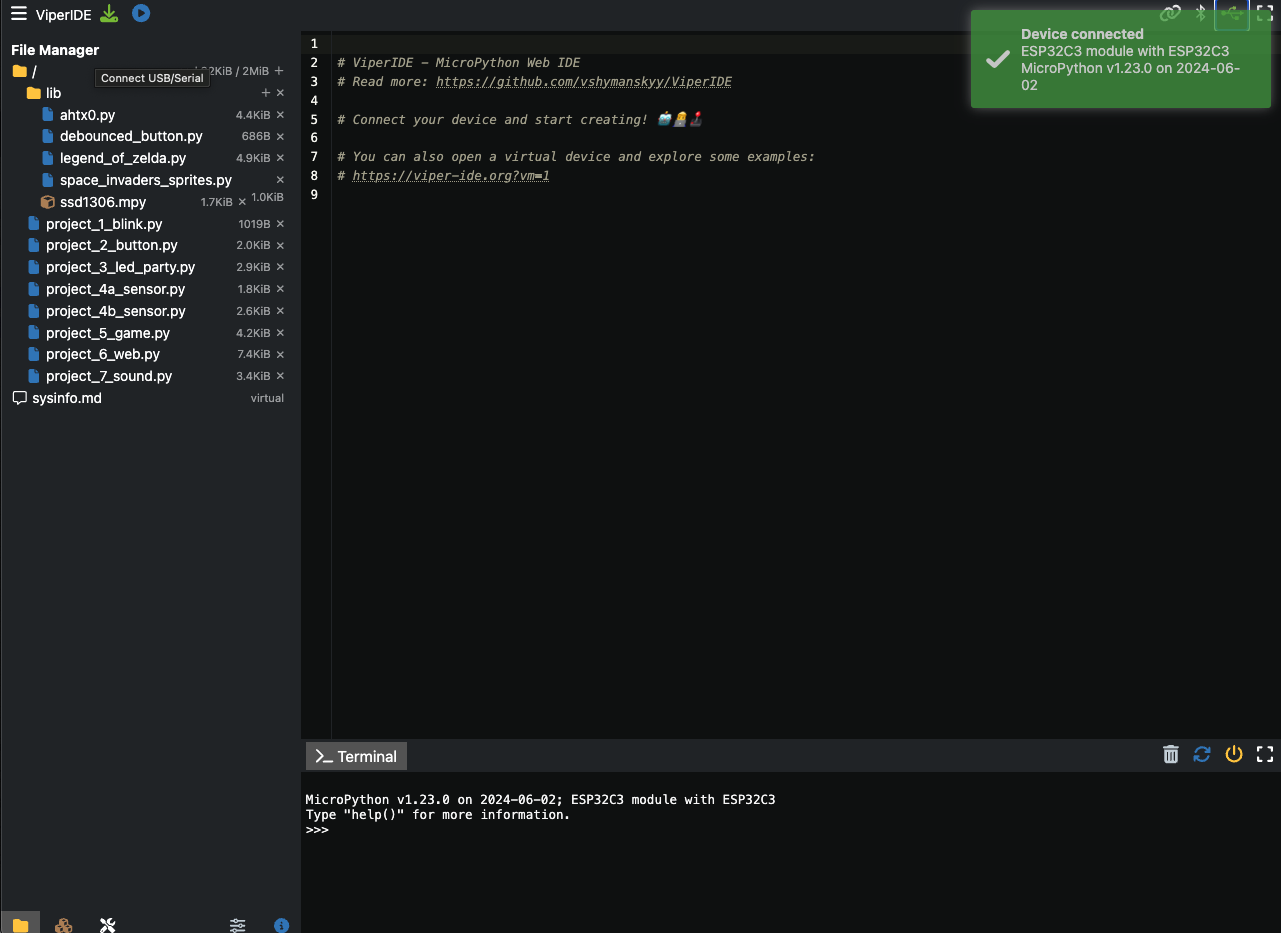
\includegraphics[width=.6\linewidth]{common/viper_connected.png}
    \caption{Make sure to open the right file for this project}
\end{figure}

Click on the file named "project\_6\_web.py". This will load the code in the editor for this section. Read through the comments
and the code to get a sense for how it works. You will need to edit the code and provide values for the WiFi network name
and password before it will work:

\begin{figure}[H]
    \centering
    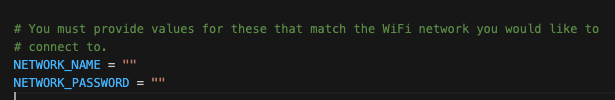
\includegraphics[width=.6\linewidth]{project_6/enter_wifi_credentials.png}
    \caption{If you are doing this during the workshop at NetApp, these will be given to you. If you are at home, use the credentials for your house.}
\end{figure}

Once you are ready, you can click the blue play button in the upper left of the window
to start the program.

You can press the left and right buttons to rotate through the different views on the screen. Note that it takes
a few seconds for the microcontroller to load and parse the data from each API. This can sometimes lead to
buggy behavior when pressing the buttons quickly.

\subsection{Examining the code}

This project's code shows a few new concepts:
\begin{itemize}
    \item Configuring the microcontroller's WiFi hardware and connecting to a network
    \item Making requests to a web-based API
    \item Parsing the results of the API and displaying them on our screen
\end{itemize}

Let's take each of these and examine them closer

\subsubsection{Connecting to WiFi}
\begin{lstlisting}[language=Python,caption=WiFi Code]
import network

# You must provide values for these that match the WiFi network you would like to
# connect to.
NETWORK_NAME = ""
NETWORK_PASSWORD = ""

def connect_to_wifi():
    if not NETWORK_NAME or not NETWORK_PASSWORD:
        print("Don't forget to fill in the WiFi details at the top of the script!")
        return False

    print(f"Connecting to {NETWORK_NAME}...")
    OLED.text("Connecting...", 12, 25)
    OLED.show()

    interface = network.WLAN(network.STA_IF)
    interface.active(True)
    interface.connect(NETWORK_NAME, NETWORK_PASSWORD)
    tries = 10
    while tries > 0:
        if not interface.isconnected():
            tries -= 1
            time.sleep(1)
        else:
            print(f"Connected to {NETWORK_NAME} successfully")
            break
    else:
        print(f"Failed to connect to {NETWORK_NAME}. Is the password correct?")
        return False

    return True
\end{lstlisting}

In the listing above, we see just the code that is responsible for setting up the WiFi hardware and connecting
to the network. First we import the network module. This is part of the standard library for MicroPython.
In the \textbf{connect\_to\_wifi()} function, we make sure the network name and password are set. Then
we print out a status message to let the user know that something is happening. Then we get the \textbf{interface}
object by asking the \textbf{network} library to give us a handle to the microcontroller's WiFi chip. We mark
the \textbf{interface} as active and tell it to connect with the credentials the user gave us.

It takes a little time to connect to the WiFi router, so we have a loop to wait until that happens. If we
get connected, then we will exit the function returning \textbf{True}. If something prevents us from conencting,
for example a mistyped password, then we will print a message to let the user know and return \textbf{False}.

\subsubsection{Talking to an API}
\begin{lstlisting}[language=Python,caption=Making Web Requests]
def draw_date_and_time():
    # Use the timeapi.io site to fetch the current time
    # using the IP address of our microcontroller
    # https://timeapi.io/swagger/index.html
    response = requests.get(f"https://timeapi.io/api/time/current/ip?ipAddress={IP_ADDRESS}")
    date_time = response.json()
    OLED.fill(0)
    OLED.text(f"{date_time['hour']:02d}:{date_time['minute']:02d}:{date_time['seconds']:02d}", 30, 5)
    OLED.text(f"{date_time['dayOfWeek']}", 35, 15)
    OLED.text(f"{date_time['date']}", 20, 25)
\end{lstlisting}

In the above code, we make use of our new network connection by making an HTTP GET request to the \url{https://timeapi.io/}
site. This site provides a JSON-based RESTful API that anyone can use. The URL that we make the request to is
asking for the current time at the IP address that we were assigned when we connected to WiFi. If we made this request
in our browser, the response would look something like this:

\begin{figure}[H]
    \centering
    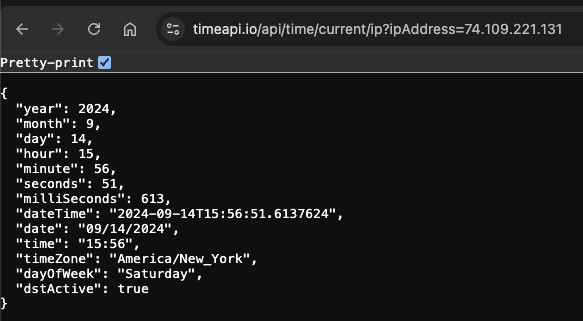
\includegraphics[width=.6\linewidth]{project_6/api_response.png}
    \caption{An example response from the timeapi.io site}
\end{figure}

This format is called JSON. It is a way of expressing groups of data that many programming languages can
understand. It is one of the most common formats for web-based APIs. In our code, we use the \textbf{response.json()}
function to parse this response into a Python dictionary object. We can then access the fields of the response in
our code and print them out on our screen.

\section{Review}
This chapter is an example of how you might create an Internet of Things device using a microcontroller and
some Python code. While our example is small, you could imagine that instead of our small screen, we are
displaying this on a large touch screen, perhaps one acting as the bathroom mirror. Then when you were getting
ready each day, the things most relevant to you would be readily visible.

\section{Possible Extensions}
If you want to do some experimentation, try these:

\begin{itemize}
    \item Change the code to auto-cycle between the screens every X seconds even without a button press
    \item Find another web-based API that is free and accessible and display information from it on a 4th screen
\end{itemize}

